\section{Введение}
Принцип эквивалентности инертной и гравитационной масс является одним из краеугольных камней общей теории относительности. Экспериментально он проявляется в независимости ускорения свободного падения от массы и состава тела. В данной работе на установке с лазерными лучами и частотомером Ч3-32 измеряется время падения шариков из шести различных материалов, и по нему вычисляется ускорение $g$.

\subsection{Цель работы}
\begin{enumerate}
    \item Проверить принцип эквивалентности масс.
    \item Измерить ускорение свободного падения.
    \item Освоить метод измерения интервалов времени частотомером-хронометром.
    \item Оценить погрешности косвенных измерений.
\end{enumerate}

\subsection{Решаемые задачи}
\begin{enumerate}
    \item Вычислить массы шариков по плотности и диаметру.
    \item Провести статистическую обработку 30 измерений времени падения для каждого материала.
    \item Рассчитать $g$ по формуле $g = 2(h - v_0 t)/t^2$.
    \item Найти погрешность $\Delta g$ методом частных производных.
    \item Сравнить полученные значения $g$ с табличным $9,81$ м/с².
\end{enumerate}

\section{Основная часть}

\subsection{Теоретическая часть}
Инертная масса $m_{\text{ин}}$ определяется через ускорение под действием силы, гравитационная $m_{\text{гр}}$ – через силу тяготения. Принцип эквивалентности утверждает $m_{\text{ин}} = m_{\text{гр}}$, откуда ускорение свободного падения не зависит от тела. Для движения с начальной скоростью $v_0$:
\begin{equation}
    h = v_0 t + \frac{gt^2}{2} \quad \Rightarrow \quad g = \frac{2(h - v_0 t)}{t^2}. \tag{1}
\end{equation}
Погрешность косвенного измерения:
\begin{equation}
    \Delta g = \sqrt{\left(\frac{\partial g}{\partial h}\Delta h\right)^2 + \left(\frac{\partial g}{\partial v_0}\Delta v_0\right)^2 + \left(\frac{\partial g}{\partial t}\Delta t\right)^2}, \tag{2}
\end{equation}
где частные производные:
\[
\frac{\partial g}{\partial h} = \frac{2}{t^2},\quad
\frac{\partial g}{\partial v_0} = -\frac{2}{t},\quad
\frac{\partial g}{\partial t} = -\frac{4(h - v_0 t)}{t^3} - \frac{2v_0}{t^2}.
\]

\subsection{Экспериментальная установка}
Схема установки приведена на рис.~\ref{fig:scheme}. Луч от квантового генератора (лазера) ЛГ направляется на призму полного внутреннего отражения П1, от неё на призму П2, а затем на фотодиод ФД. При отодвигании заслонки З шарик, находящийся в трубке Т, падает в лузу Л и пересекает два световых луча, расстояние между которыми $h = (0,272 \pm 0,001)$ м. Когда шарик пересекает верхний луч, фотодиод ФД вырабатывает импульс, который после усиления подаётся на вход частотомера Ч3-32 и запускает его. При пересечении шариком нижнего луча импульс останавливает счёт. Начальная скорость шарика в момент пересечения верхнего луча $v_0 = (1,050 \pm 0,005)$ м/с задаётся конструкцией установки. Диаметр всех шариков $d = 10$ мм.

\begin{figure}[ht!]
    \centering
    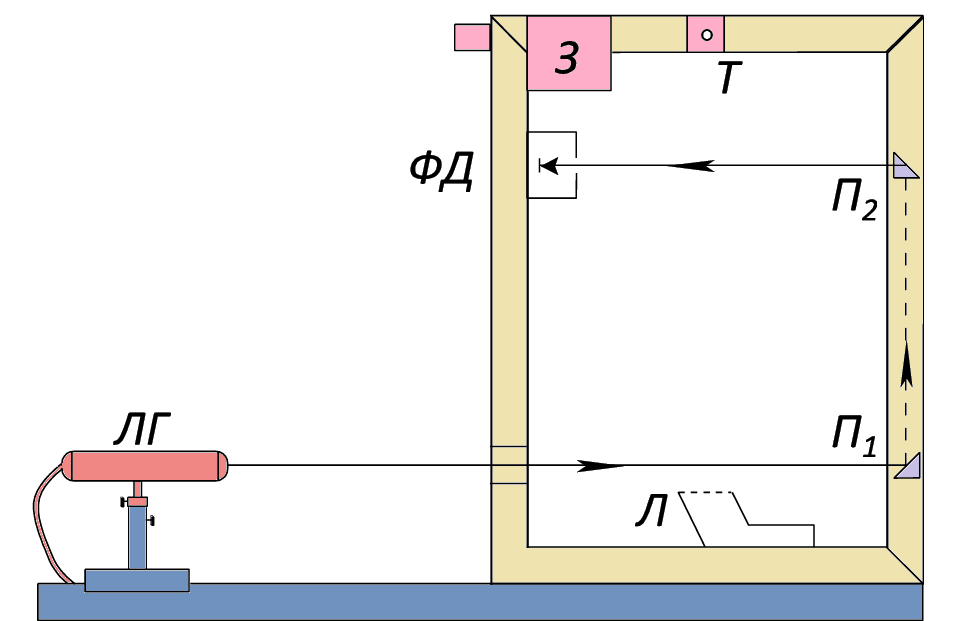
\includegraphics[width=0.6\textwidth]{Scheme.png}
    \caption{Схема экспериментальной установки}
    \label{fig:scheme}
\end{figure}

Фотография реальной установки представлена на рис.~\ref{fig:device}. На ней видны лазер, частотомер, блок питания и трубка с шариками.

\begin{figure}[ht!]
    \centering
    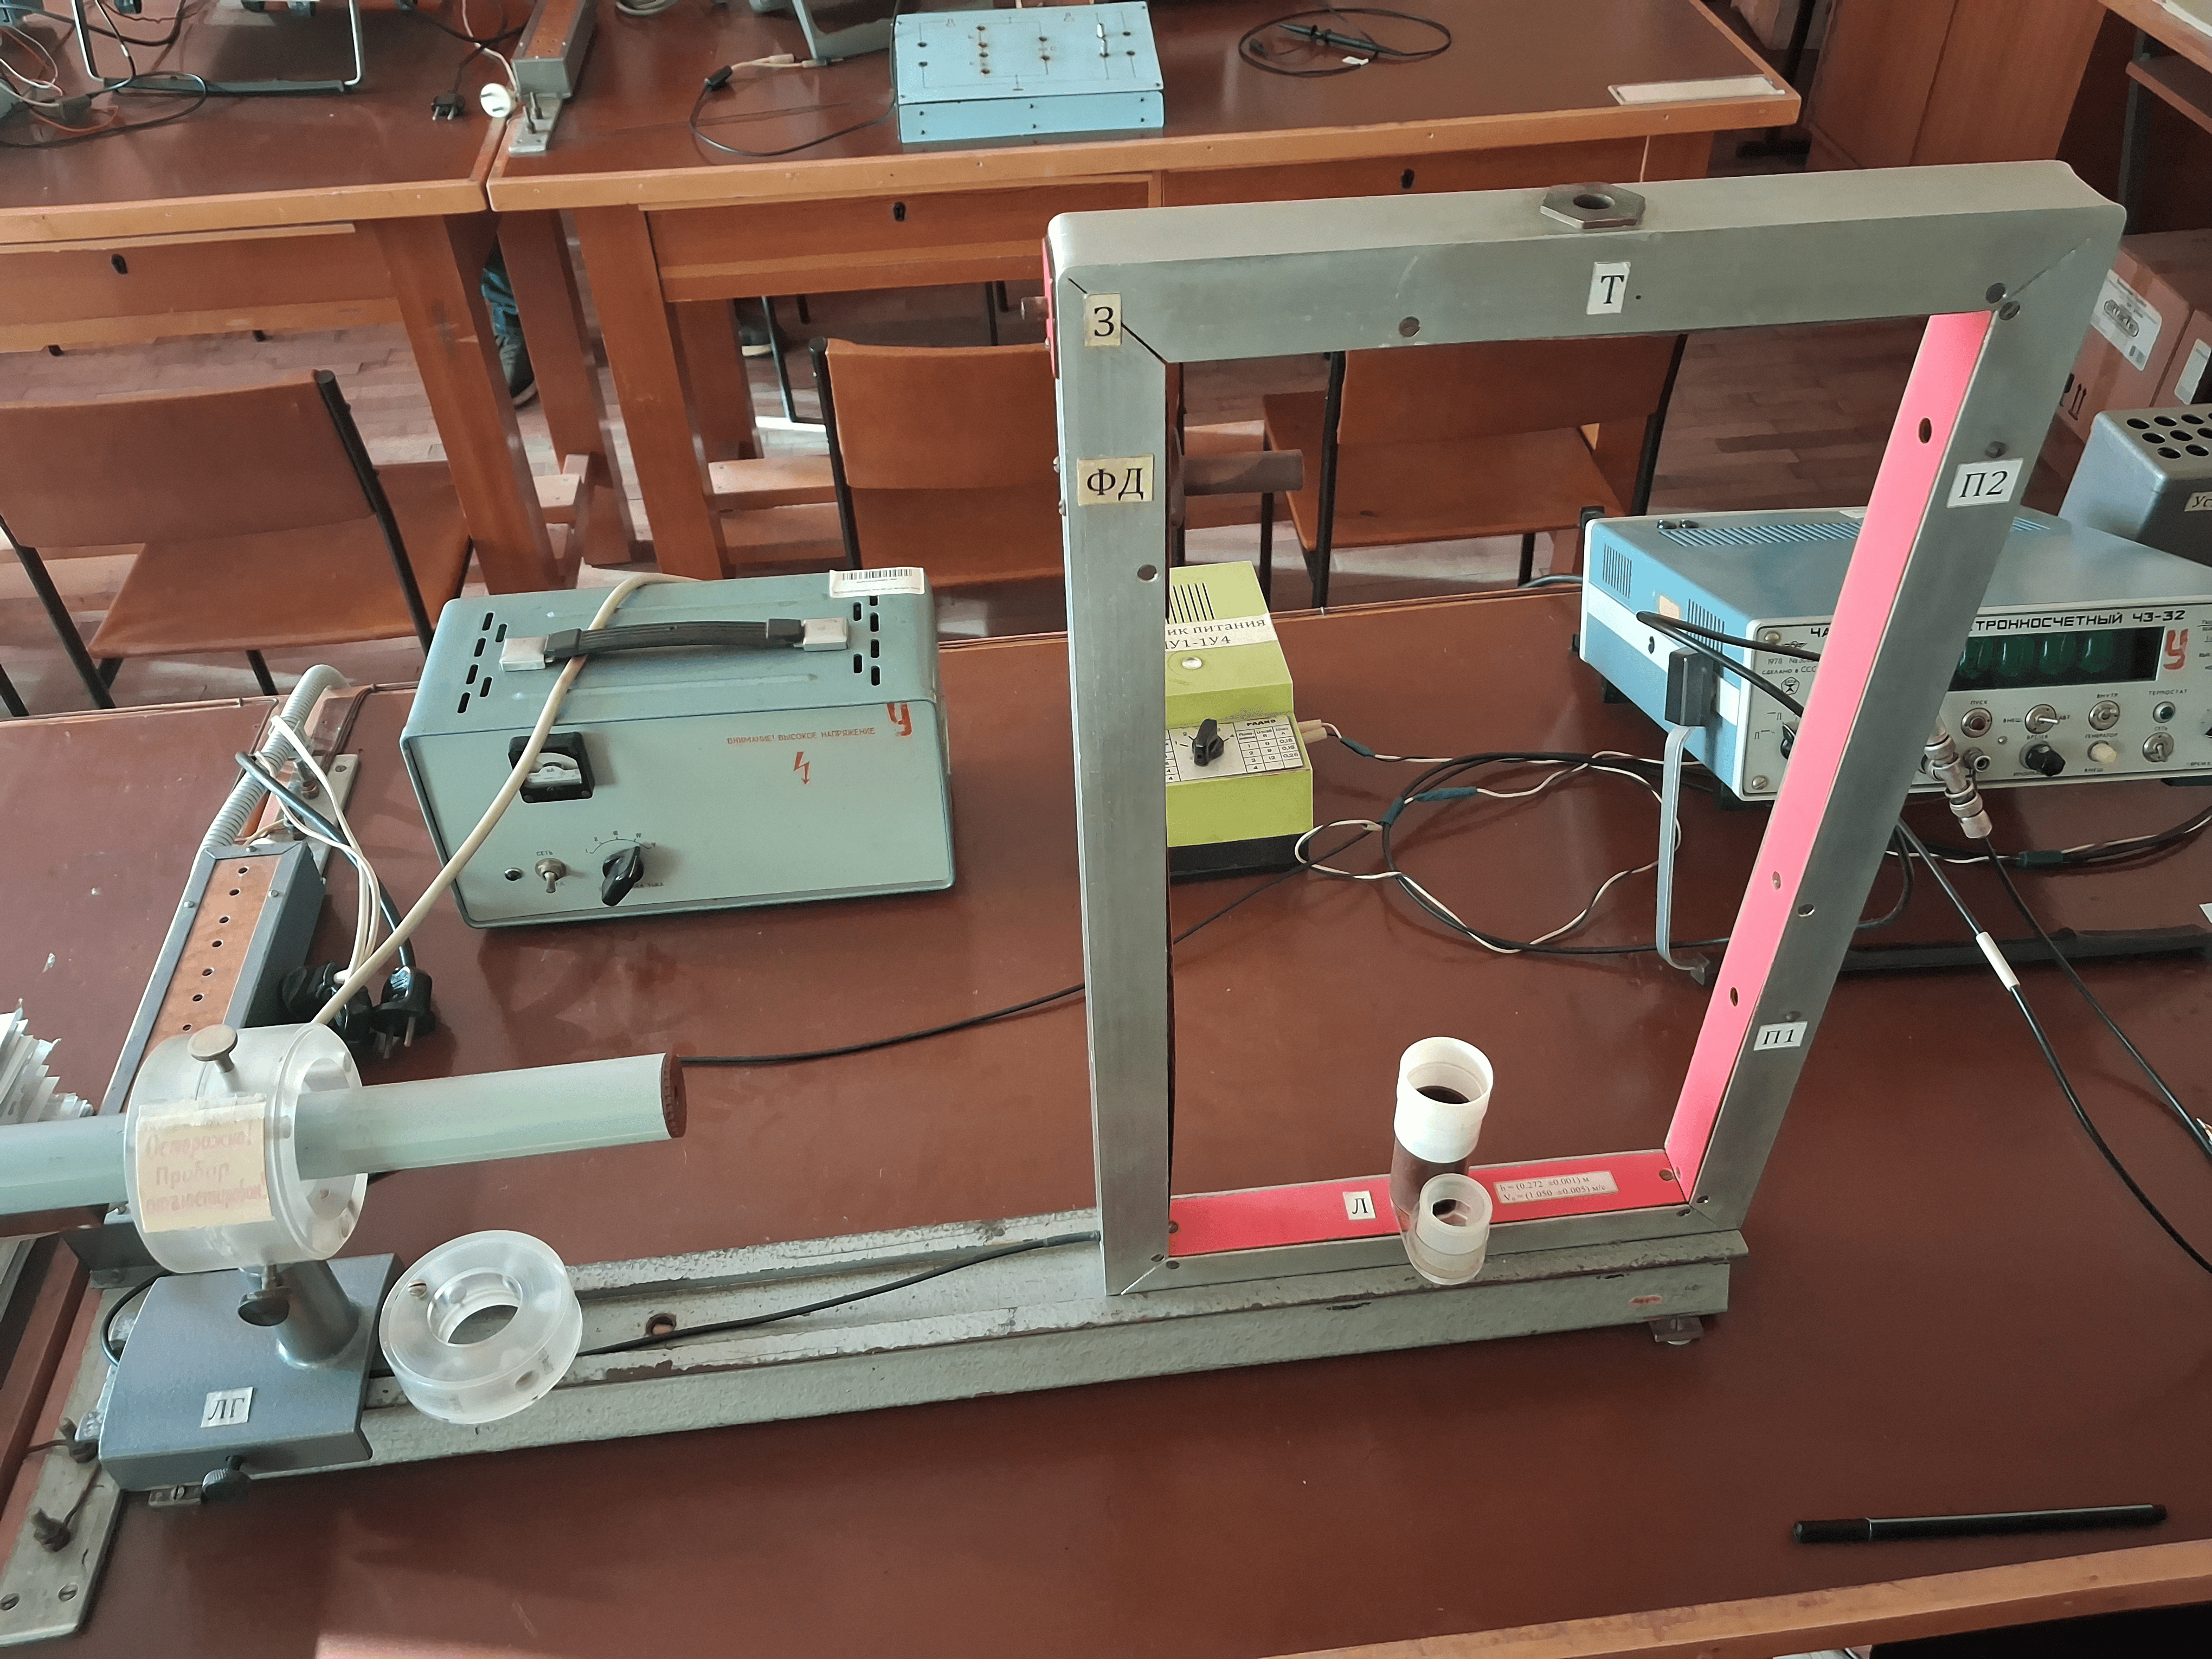
\includegraphics[width=0.6\textwidth]{Device.png}
    \caption{Фотография экспериментальной установки}
    \label{fig:device}
\end{figure}
\subsection{Результаты измерений и их обработка}

\subsubsection{Таблица 1. Масса шариков}
Масса вычисляется по формуле $m = \rho \cdot \frac{4}{3}\pi (d/2)^3$. Результаты сведены в табл.~\ref{tab:masses}.

\begin{table}[ht!]
\centering
\caption{Масса шариков}
\label{tab:masses}
\begin{tabular}{|c|c|c|c|}
\hline
Вещество & Плотность, г/см³ & Диаметр, м & Масса, кг \\
\hline
Алюминий & 2,79 & 0,01 & $1,461\cdot10^{-3}$ \\
Латунь   & 8,50 & 0,01 & $4,451\cdot10^{-3}$ \\
Сталь    & 7,90 & 0,01 & $4,136\cdot10^{-3}$ \\
Дерево   & 0,71 & 0,01 & $3,718\cdot10^{-4}$ \\
Плексиглас & 1,18 & 0,01 & $6,178\cdot10^{-4}$ \\
Свинец   & 11,34 & 0,01 & $5,938\cdot10^{-3}$ \\
\hline
\end{tabular}
\end{table}

\subsubsection{Таблица 2. Время падения шариков (30 измерений)}
Для каждого материала проведено $n=30$ измерений времени $t_i$ (в миллисекундах). Исходные данные представлены в табл.~\ref{tab:rawtime}. В последней строке приведены средние значения $\bar{t}$ для каждого материала.

{\tiny
\begin{longtable}{|c|c|c|c|c|c|c|}
\hline
№ п/п & Алюминий & Латунь & Сталь & Дерево & Плексиглас & Свинец \\
\hline
1 & 149,679 & 150,104 & 149,275 & 150,694 & 150,660 & 149,847 \\
2 & 150,168 & 149,840 & 149,657 & 150,770 & 150,539 & 150,106 \\
3 & 152,644 & 149,983 & 149,945 & 151,824 & 150,370 & 150,138 \\
4 & 150,115 & 150,354 & 150,128 & 151,097 & 150,800 & 149,704 \\
5 & 149,902 & 149,941 & 150,363 & 151,005 & 150,504 & 150,288 \\
6 & 150,628 & 149,961 & 150,187 & 151,734 & 150,509 & 150,257 \\
7 & 150,852 & 150,183 & 149,895 & 151,320 & 150,697 & 150,000 \\
8 & 150,584 & 150,049 & 149,869 & 150,818 & 151,150 & 149,949 \\
9 & 150,227 & 149,914 & 149,758 & 150,995 & 150,446 & 150,190 \\
10 & 150,502 & 150,106 & 149,968 & 151,199 & 150,633 & 149,759 \\
11 & 149,977 & 149,920 & 150,331 & 151,194 & 150,551 & 150,429 \\
12 & 150,113 & 150,117 & 149,886 & 150,876 & 151,033 & 149,901 \\
13 & 150,626 & 149,821 & 150,296 & 152,212 & 151,848 & 150,169 \\
14 & 150,205 & 150,409 & 149,761 & 151,662 & 151,395 & 150,424 \\
15 & 150,359 & 149,890 & 149,715 & 151,241 & 150,954 & 149,799 \\
16 & 150,112 & 150,277 & 150,928 & 150,859 & 150,696 & 149,842 \\
17 & 150,124 & 149,836 & 149,986 & 150,969 & 150,518 & 149,937 \\
18 & 151,217 & 149,655 & 150,019 & 151,590 & 150,700 & 150,805 \\
19 & 150,604 & 150,048 & 149,828 & 150,997 & 150,649 & 150,590 \\
20 & 149,930 & 150,099 & 149,904 & 150,917 & 150,554 & 150,672 \\
21 & 151,423 & 151,118 & 149,368 & 151,406 & 150,564 & 150,339 \\
22 & 151,129 & 150,874 & 149,822 & 151,263 & 150,566 & 149,917 \\
23 & 150,081 & 150,536 & 149,913 & 151,623 & 151,222 & 149,951 \\
24 & 150,518 & 150,615 & 150,148 & 151,285 & 150,956 & 150,259 \\
25 & 150,678 & 150,426 & 149,736 & 150,984 & 151,195 & 150,107 \\
26 & 149,977 & 150,202 & 149,813 & 151,509 & 150,891 & 149,851 \\
27 & 150,569 & 149,907 & 149,947 & 151,279 & 151,058 & 149,939 \\
28 & 150,376 & 150,037 & 149,812 & 150,922 & 150,540 & 150,000 \\
29 & 151,060 & 149,823 & 150,091 & 151,513 & 150,955 & 150,971 \\
30 & 150,294 & 150,776 & 149,834 & 150,959 & 150,353 & 149,897 \\
\hline
Среднее & 150,489 & 150,161 & 149,939 & 151,224 & 150,784 & 150,135 \\
\hline
\caption{Время падения шариков $t$, мс}
\label{tab:rawtime}
\end{longtable}
}

\subsubsection{Таблица 3. Погрешность времени $\Delta t$}
Для каждого материала вычислены:
\begin{itemize}
    \item среднее арифметическое $\bar{t}$ (переведено в секунды);
    \item стандартное отклонение выборки $s_t = \sqrt{\frac{1}{n-1}\sum (t_i-\bar{t})^2}$;
    \item стандартная ошибка среднего $s_{\bar{t}} = s_t/\sqrt{n}$;
    \item случайная погрешность $\Delta t_{\text{случ}} = t_{\alpha,n-1}\cdot s_{\bar{t}}$ (коэффициент Стьюдента $t_{0,95;29}=2,042$);
    \item приборная погрешность частотомера $\Delta t_{\text{приб}} = 0,001$ мс, приведённая к стандартной неопределённости $\Delta t_{\text{приб}}/3$;
    \item полная погрешность $\Delta t = \sqrt{(\Delta t_{\text{случ}})^2 + (\Delta t_{\text{приб}}/3)^2}$.
\end{itemize}
Результаты представлены в табл.~\ref{tab:deltat}.

\begin{table}[ht!]
\centering
\caption{Погрешность измерения времени $\Delta t$}
\label{tab:deltat}
\begin{tabular}{|c|c|}
\hline
Вещество & $\Delta t$, с \\
\hline
Алюминий   & $2,178\cdot10^{-4}$ \\
Латунь     & $1,287\cdot10^{-4}$ \\
Сталь      & $1,137\cdot10^{-4}$ \\
Дерево     & $1,341\cdot10^{-4}$ \\
Плексиглас & $1,264\cdot10^{-4}$ \\
Свинец     & $1,188\cdot10^{-4}$ \\
\hline
\end{tabular}
\end{table}

\subsubsection{Таблица 4. Ускорение свободного падения $g$}
По формуле (1) с использованием $\bar{t}$ (в секундах) рассчитаны значения $g$ для каждого материала. Результаты приведены в табл.~\ref{tab:g}.

\begin{table}[ht!]
\centering
\caption{Ускорение свободного падения}
\label{tab:g}
\begin{tabular}{|c|c|}
\hline
Вещество & $g$, м/с² \\
\hline
Алюминий   & 10,066 \\
Латунь     & 10,141 \\
Сталь      & 10,192 \\
Дерево     & 9,901  \\
Плексиглас & 10,000 \\
Свинец     & 10,147 \\
\hline
\end{tabular}
\end{table}

\subsubsection{Таблица 5. Погрешность $\Delta g$}
Погрешность $\Delta g$ вычислена по формуле (2) с использованием частных производных. Результаты приведены в табл.~\ref{tab:dg}.

\begin{table}[ht!]
\centering
\caption{Погрешность измерения ускорения свободного падения}
\label{tab:dg}
\begin{tabular}{|c|c|}
\hline
Вещество & $\Delta g$, м/с² \\
\hline
Алюминий   & 0,121 \\
Латунь     & 0,115 \\
Сталь      & 0,114 \\
Дерево     & 0,114 \\
Плексиглас & 0,114 \\
Свинец     & 0,114 \\
\hline
\end{tabular}
\end{table}

\subsection{Обсуждение результатов}
Все полученные значения $g$ лежат в интервале от $9,90$ до $10,19$ м/с². Теоретическое значение $g_{\text{табл}} = 9,81$ м/с² попадает в доверительные интервалы для всех материалов: 
\begin{itemize}
    \item Алюминий: $10,07 \pm 0,12$,
    \item Латунь: $10,14 \pm 0,11$,
    \item Сталь: $10,19 \pm 0,11$,
    \item Дерево: $9,90 \pm 0,11$,
    \item Плексиглас: $10,00 \pm 0,11$,
    \item Свинец: $10,15 \pm 0,11$.
\end{itemize}
Таким образом, в пределах погрешностей ускорение свободного падения не зависит от материала шариков, что подтверждает принцип эквивалентности масс. Небольшое систематическое завышение $g$ (около $0,2$–$0,4$ м/с²) может быть связано с неточностью задания $v_0$ или $h$, а также с влиянием сопротивления воздуха.

\subsection{Анализ систематических погрешностей}
Возможные источники систематических ошибок:
\begin{itemize}
    \item Сопротивление воздуха – для лёгких шариков (дерево, плексиглас) оно может немного занижать $g$, но вклад не превышает $0,1$ м/с².
    \item Непараллельность лазерных лучей – приводит к ошибке в измерении $h$.
    \item Задержки срабатывания фотодиода и электроники – добавляют постоянную составляющую к измеряемому интервалу.
    \item Неточность паспортного значения $v_0$ – может давать смещение $g$.
\end{itemize}
Однако все эти эффекты не меняют основного вывода о независимости $g$ от материала.

\section{Выводы}
\begin{enumerate}
    \item Экспериментально подтверждена независимость ускорения свободного падения от материала падающих тел (в пределах погрешностей).
    \item Измеренные значения $g$ для шести материалов находятся в интервале $9,90$–$10,19$ м/с² и согласуются с табличным $9,81$ м/с².
    \item Освоена методика статистической обработки многократных измерений времени и расчёта погрешностей косвенных измерений.
    \item Выявлено, что случайная погрешность времени полностью доминирует над приборной погрешностью частотомера.
\end{enumerate}